\documentclass[aps,prl,twocolumn,superscriptaddress,nofootinbib,floatfix]{revtex4-2}
\usepackage{amsmath,amssymb}
\usepackage{graphicx}
\usepackage[colorlinks=true,allcolors=blue]{hyperref}
% macros.tex -- shared by letter.tex and supplement.tex.
% Headline switch: \HLJclosedfalse quotes Delta_g = 1000 (the near-gap large-spin hypothesis at Delta_g = 300 is open);
% \HLJclosedtrue would quote Delta_g = 300 (then also set \HLJgrade and \HLJsource).
\newif\ifHLJclosed
\HLJclosedfalse
\newcommand{\HLJgrade}{[grade]}
\newcommand{\HLJsource}{Supplemental Material}

\newcommand{\DgHead}{\ifHLJclosed 300\else 1000\fi}
\newcommand{\CubicHead}{\ifHLJclosed 3.13\times10^{-6}\else 2.89\times10^{-8}\fi}
\newcommand{\QuartHead}{\ifHLJclosed 72.0\else 92.8\fi}
\newcommand{\QuartRep}{\ifHLJclosed 125.7\else 164.5\fi}
\newcommand{\GthreeHead}{\ifHLJclosed 104\else 120\fi}
\newcommand{\HLJwindowGrade}{\ifHLJclosed \HLJgrade\else [I]\fi}

\newcommand{\HLJstatusLetter}{\ifHLJclosed The near-gap large-spin states at $\Delta_g=300$ are
covered at grade \HLJgrade\ (\HLJsource), so we quote $\Delta_g=300$.\else We quote $\Delta_g=1000$
because at $\Delta_g=300$ positivity on near-gap states of large spin is an open hypothesis.\fi}


\begin{document}

\title{Energy Detectors Bound Non-Einstein Gravity by the Inverse Cube of the Higher-Spin Gap}

\author{Ansh Mishra}
\email{ansh.mishra2025@gmail.com}
\affiliation{Independent researcher}
\author{Aryan Senthilkumar}
\email{aryan.senthilk@gmail.com}
\affiliation{Independent researcher}

\date{\today}

\begin{abstract}
In a three-dimensional conformal field theory the stress-tensor three-point function has two coefficients that vanish for Einstein
gravity, $t_4$ and the parity-odd $\alpha_T$. In theories with a large central charge and a gap $\Delta_g$ in the spectrum of higher-spin
single-trace operators, they are expected to fall as $\log\Delta_g/\Delta_g^4$, but the only rigorous bound that needs no positivity
assumption fell as $1/\Delta_g$. Using only the commutativity of energy detectors at every angular harmonic, we prove
$(t_4^2+\alpha_T^2)^{1/2}\le994/\Delta_g^3$ asymptotically, with an explicit bound at every gap, for instance $9.9\times10^{-7}$ at
$\Delta_g=1000$. The proof rests on a hypergeometric dual that we show to be feasible on every heavy state and on every allowed light
single trace. The same rules cannot reach beyond $588/\Delta_g^3$. The bound holds at leading order in the inverse central charge: light
multi-trace states enter with a coefficient that grows exponentially with the gap.
\end{abstract}

\maketitle

\textit{Introduction}---A conformal field theory (CFT) with a large central charge $c_T$ and a large gap $\Delta_g$ in its spectrum of
higher-spin single-trace operators is expected to be dual to nearly Einstein gravity~\cite{HPPS,CEMZ,AHKT}. In three dimensions the
stress-tensor three-point function $\langle TTT\rangle$ is fixed by $c_T$ and two numbers~\cite{HofmanMaldacena,Buchel,CDPrakash,GPY}:
$t_4$, and a parity-odd coefficient $\alpha_T$ that exists only in three dimensions. Both vanish for Einstein gravity, and we write
$\tau=(t_4^2+\alpha_T^2)^{1/2}$ for the deviation. In the bulk $\tau=240|\hat g_3|$, where $\hat g_3$ is the $R^3$ coupling of
Ref.~\cite{CHLPS}. Every unitary CFT$_3$ has $\tau\le4$, the conformal collider bound~\cite{HofmanMaldacena,CDPrakash}.

How small must $\tau$ be at a given gap? Causality arguments give $\tau\lesssim\log\Delta_g/\Delta_g^4$ parametrically~\cite{AKT,MeltzerPerlmutter,CEMZ},
and sum rules from the commutativity of energy detectors force $t_4\to0$ as the gap grows~\cite{KKSDZ,BHM}. Dispersive sum rules give
explicit constants in flat space~\cite{CHLPS} and, with positivity of a functional on heavy states, in AdS~\cite{CHMRS,CLSD}. The
only bound with explicit constants that needs no positivity input was~\cite{SM}
\begin{equation}
\tau\le\tau_*(\Delta_g)=\frac{160}{9(\Delta_g-2)}\Big[1-\frac{49}{(2\Delta_g+9)^2}\Big]^{-1/2},
\label{eq:taustar}
\end{equation}
three powers of $\Delta_g$ weaker than expected.

Here we show that the same input, commutativity of energy detectors, gives a bound falling as $\Delta_g^{-3}$, with explicit constants at
every gap (Fig.~\ref{fig:bounds}). The improvement comes from using every angular harmonic of the detector commutator rather than one.
The resulting linear program has a dual whose feasibility on the infinite set of heavy states we prove analytically. We also show
which part of the problem stops further progress: these rules cannot do better than $588/\Delta_g^3$, and light multi-trace states,
which we control only in the planar limit, enter with large coefficients. We write ``we prove'' or ``we derive'' for a written argument,
``certified'' for a computer-assisted proof in exact or interval arithmetic, and ``we sketch'' for an argument whose details are
incomplete; the Supplemental Material~\cite{SM} grades every statement on this scale.

\begin{figure}[tb]
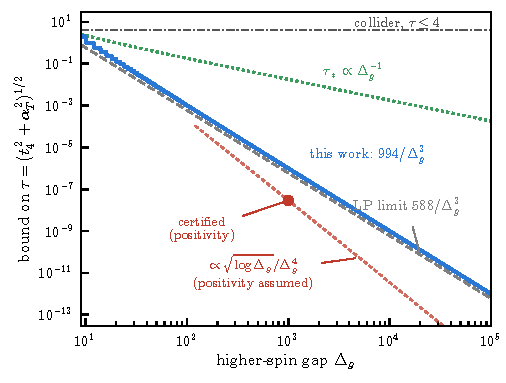
\includegraphics[width=\columnwidth]{fig/fig_angular}
\caption{\label{fig:bounds}Bounds on $\tau=(t_4^2+\alpha_T^2)^{1/2}$ against the higher-spin gap, at leading order in $1/c_T$.
Dot-dashed: the collider bound. Green dotted: the earlier positivity-free bound $\tau_*$, Eq.~\eqref{eq:taustar}, whose error terms carry
no large constants. Blue: this work, Eq.~\eqref{eq:main}, exact at each gap (the steps come from $n=\lfloor\Delta_g/2\rfloor$). Grey
dashed: the limit $588/\Delta_g^3$ of the same rules. Red: the dispersive bound of Eq.~\eqref{eq:cubic}, certified at $\Delta_g=1000$
(filled circle); the red dashed curve is the same functional at its own gap with positivity assumed, for orientation only.}
\end{figure}

\textit{Assumptions}---We take $c_T$ large and assume: (i)~\emph{a higher-spin gap}, so every single-trace operator of spin four or
more in $T\times T$ has twist at least $\Delta_g$, while single traces of spin zero and two may be light; (ii)~\emph{weak coupling below
the gap}: as $c_T\to\infty$ at fixed $\Delta_g$, the OPE of the unit-normalized $T$ with itself below the gap is that of a generalized
free field, with double-trace anomalous dimensions $o(c_T^{-1/2})$ and other squared OPE coefficients $o(1/c_T)$, uniformly in spin.
Large-$N$ factorization gives (ii) at each fixed spin; the uniformity is the assumption. It holds for tree-level Einstein gravity in
AdS$_4$~\cite{SM}, and no bulk effective theory is assumed. We also use three inputs of Eq.~\eqref{eq:taustar}: the light-ray detector
identities hold as operator identities, a mixed detector commutator converges in the light-cone limit as assumed in
Ref.~\cite{KKSDZ}, and no scalar of dimension at most one appears in $T\times T$. No positivity of any functional is assumed. Our
statements hold at leading order in $1/c_T$; we return to what this means below.

\textit{Energy detectors at every harmonic}---Light-transformed stress tensors act as energy detectors
$E(\varphi)$~\cite{KSDlight,HofmanMaldacena}, and detectors at different directions commute~\cite{KKSDZ}. Consider the state created by
$T$ at rest with helicity $+2$, and the angular modes $E_m=\int d\varphi\,e^{im\varphi}E(\varphi)/E$. Rotation covariance sends this
state under $E_m$ to states of $SO(2)$ charge $2+m$. The rest-frame amplitudes of an intermediate primary $\mathcal O$ of spin $J$ and
dimension $\Delta$ lie on two helicity ladders, $b=0$ and $b=4$, and conservation of the light-transformed $T$ fixes the ladder ratios
$r_k^{(b)}(J,\Delta)=|a_{\mathcal O,b,k}|^2/|a_{\mathcal O,b,0}|^2$ exactly~\cite{SM}. The stress tensor itself carries only charges $\pm2$,
and its weight in the fourth harmonic is fixed by $\langle TTT\rangle$, $|c|^2=\tau^2/16$. Inserting a complete set of states into
$\langle T|[E_m,E_{-m}]|T\rangle=0$ gives one exact rule for every $m=k+2$,
\begin{equation}
\sum_{\mathcal O}\rho^{(4)}_{\mathcal O}r_k^{(4)}-\sum_{\mathcal O\neq T}\rho^{(0)}_{\mathcal O}r_k^{(0)}=\delta_{k2}\,\frac{\tau^2}{16},
\label{eq:Rk}
\end{equation}
with $\rho^{(b)}_{\mathcal O}=|a_{\mathcal O,b,0}|^2\ge0$. Earlier work used only $k=2$, with the second sum dropped; that gives
Eq.~\eqref{eq:taustar}. The other rules balance the two ladders against each other. We derive Eq.~\eqref{eq:Rk} from the same
commutativity input, and we check it in free fields, where both sides are computable state by state~\cite{SM}. A second exact sum rule, from
commutativity of a detector with its first moment in retarded time, fixes the total weight,
$\sum_{\mathcal O\neq T,b}W_b(\Delta)\rho^{(b)}_{\mathcal O}=3$ with $W_b=[(\Delta-1)(\Delta-2)-b(b-1)]/3+\tfrac32$~\cite{SM}.

\textit{The bound}---Multiplying the $k$-th rule by $\lambda_k$ and adding the weight sum rule turns the problem into a linear program.
If, for every state that can appear, $W_4+\sum_k\lambda_kr^{(4)}_k\ge0$ and $W_0-\sum_k\lambda_kr^{(0)}_k\ge0$, then $\tau^2\le48/(-\lambda_2)$.
We take $\lambda_k\binom{k+3}3^2=-A\,(-n)_k(n)_k/(k!)^2$ with $n=\lfloor\Delta_g/2\rfloor$. The two conditions then involve a terminating
hypergeometric sum $R_{n,b}(J,\Delta)={}_4F_3(-n,n,b-J,J+b+1;1,b+2-\Delta,\Delta+b-1;1)$, which for large $n$ is a sum of terms of size
$e^{2n}$ with cancellations among them.

We prove that the dual is feasible on every heavy state, every spin $J$ on both ladders and every real $\Delta\ge J+\Delta_g$, for every real
$\Delta_g\ge4$. The key is an exact three-term recurrence of $R_{n,b}$ in the spin, valid at real $\Delta$. On the $b=0$ ladder a quadratic
energy decreases along the recurrence; on the $b=4$ ladder a weighted (Sonin) energy does. This reduces the infinitely many states to
a single fixed-degree polynomial inequality, which we certify with 338 positive integer coefficients, together with explicit
certificates for the five lowest spins~\cite{SM}. An independent audit re-derived every step with separate code.

Assumption (i) allows light single traces of spin zero and two, which enter only the $b=0$ ladder. The weight $A=3(\sqrt2-1)n^2$ makes
the dual feasible on all of them, exactly: for spin two the condition is a positive square times a positive factor plus a quadratic with
negative discriminant, and it becomes tangent at $\Delta\approx0.66\,\Delta_g$, so the weight cannot be raised at leading order. The result is
\begin{equation}
\tau\le\frac{80}{\sqrt{\sqrt2-1}\;n^2\sqrt{n^2-1}}\ \xrightarrow{\ \Delta_g\to\infty\ }\ \frac{994.4}{\Delta_g^3},
\label{eq:main}
\end{equation}
with $n=\lfloor\Delta_g/2\rfloor$. It is below the collider bound for $\Delta_g>8.01$. Because $n$ is an integer, $\tau\Delta_g^3$ is larger at finite gap: it is at most
$1754$ for $\Delta_g\ge10$, $1056$ for $\Delta_g\ge100$ and $1001$ for $\Delta_g\ge1000$. At $\Delta_g=1000$ Eq.~\eqref{eq:main} gives
$\tau\le9.9\times10^{-7}$, against $0.018$ from Eq.~\eqref{eq:taustar}. In terms of the bulk coupling, $|\hat g_3|\Delta_g^3\lesssim4.1$.

\textit{What limits the power}---Three states at the gap, of spins two, four and six, satisfy every rule of Eq.~\eqref{eq:Rk} except
$k=2$ and the weight sum rule with $\tau\Delta_g^3\to4\sqrt{21600}\approx588$; we prove this exactly~\cite{SM}. No combination of these
rules can therefore do better than $\approx588/\Delta_g^3$, and with light spin-two single traces admitted the limit is $\approx694/\Delta_g^3$,
so Eq.~\eqref{eq:main} is within a factor $1.43$ of what the rules allow. We also derived further exact identities from the commutator of a
detector with its first moment: one rule for each harmonic, and rules in the helicity-flip channel, among them two parity-weighted sum
rules~\cite{SM}. In numerical linear programs they improve the constant by factors that tend to one as the gap grows. Reaching the
expected $\Delta_g^{-4}$ therefore needs input beyond commutators of detectors in states created by $T$: positivity, or data on
transitions between heavy states.

\textit{The planar limit}---The rules of Eq.~\eqref{eq:Rk} also receive contributions from light multi-trace states, chiefly double traces
$[TT]$ below the gap. By assumption (ii) their total weight vanishes as $c_T\to\infty$ at fixed $\Delta_g$, which is the sense in which
Eq.~\eqref{eq:main} holds. Their coefficient in the dual is not small, however: it reaches $10^{17}$ per unit weight at $\Delta_g=40$ and
grows exponentially with the gap~\cite{SM}. For Eq.~\eqref{eq:main} to bound the actual $\tau$, the light weight must be exponentially small
in $\Delta_g$. Equation~\eqref{eq:taustar} has no such constant: its light remainder is at most $70$ times the light weight. If the
coefficient of the light states is capped at a power of the gap, numerical linear programs give an intermediate scaling, between
$\Delta_g^{-1.2}$ and $\Delta_g^{-1.4}$~\cite{SM}. Bounding the light remainder collectively, for the full correlator rather than state by
state, would remove this caveat; we have not done so.

\textit{A dispersive bound}---A different sum rule gives a stronger bound at large gap if positivity is available. The double commutator of
detectors, integrated against a weight, gives $\sum_{\rm heavy}(\text{OPE coefficient})^2\,\Omega=-\Omega(\text{light})$~\cite{KKSDZ,CLSD,CHMRS};
if the functional $\Omega$ is positive on every heavy state, the light side is negative, and with no light single trace in $T\times T$
\begin{equation}
\tau\le2.89\times10^{-8}\qquad(\Delta_g\ge1000).
\label{eq:cubic}
\end{equation}
We certify the positivity on every heavy state at $\Delta_g=1000$, in exact and interval arithmetic~\cite{SM}. A theory with a larger gap also
has a gap of 1000, so Eq.~\eqref{eq:cubic} covers it. Its light side has the same character as above, with a coefficient
$\sim e^{\pi\Lambda/2}$, $\Lambda^2=(\Delta_g-1)(\Delta_g-2)$; for the lowest-twist double traces it is not defined state by state, and we
treat that sector with the assumption of Refs.~\cite{CHMRS,CLSD} that the light side is that of a tree-level bulk theory. At
$\Delta_g=1000$ Eq.~\eqref{eq:cubic} is 34 times stronger than Eq.~\eqref{eq:main}, but it needs certified positivity at each gap and no light
single traces, while Eq.~\eqref{eq:main} needs neither.

\textit{A thermal readout}---The deviation $\tau$ is also a thermal observable. Let $\mathcal S_E$ and $\mathcal S_H$ be the frequency-integrated
spectral weights of the stress tensor at zero momentum in the shear and Hall channels, in units of the energy density. The known shear
sum rule~\cite{Chowdhury:2016hjy} and a Hall-channel counterpart that we derive give $\mathcal S_E-\tfrac38+i\sigma\mathcal S_H=(t_4+i\alpha_T)/32$,
with $\sigma=\pm1$ a convention, in theories without light scalars that have thermal expectation values~\cite{SM,Lucas:2017dqa}. We check the
Hall coefficient exactly in large-$N$ Chern--Simons--fermion theory~\cite{Ghosh:2019sqf} and on the AdS$_4$ black brane. A measured deviation
$\delta=|\mathcal S_E-\tfrac38+i\sigma\mathcal S_H|=\tau/32$ therefore bounds the gap. Equation~\eqref{eq:taustar} gives
$\Delta_g\le2.24+5/(9\delta)$ with no large constants, and Eq.~\eqref{eq:main} gives $\Delta_g<3.21\,\delta^{-1/3}$ for $\delta\le3\times10^{-5}$
in the planar limit: a deviation of $10^{-9}$ requires a higher-spin single trace in $T\times T$ below twist about $3200$.

\textit{What is not yet a theorem}---The light multi-trace remainder of Eq.~\eqref{eq:main} is controlled only as $c_T\to\infty$, with an
exponentially large coefficient; the same is true of Eq.~\eqref{eq:cubic}, whose lowest-twist sector we also assume. The uniformity in (ii) is
an assumption, checked on tree-level Einstein gravity. The detector identities and the light-cone convergence of the mixed commutator are
inputs shared by Eqs.~\eqref{eq:taustar} and~\eqref{eq:main}. That the first-moment identities improve only the constant is numerical evidence.

\textit{Conclusions}---Commutativity of energy detectors, used at every angular harmonic, bounds the non-Einstein part of
$\langle TTT\rangle$ as $\Delta_g^{-3}$ with explicit constants and without positivity, one power short of the parametric expectation. The
power is the most these rules allow, up to a factor $1.43$ in the constant. Two obstacles remain on the way to an explicit
$\Delta_g^{-4}$ bound for theories at finite central charge: the rules themselves, which need new input beyond commutators in states created
by $T$, and the light multi-trace states, which need to be controlled collectively rather than one at a time.

\textit{Acknowledgments}---AI (Claude) assisted with the formulation and drafting of this manuscript. The authors take full
responsibility for the work presented, and have thoroughly reviewed all output.

\textit{Data availability}---The functional weights, the certificates with their inputs and outputs, and the
code that reproduces every constant are openly available~\cite{Zenodo}. The continuum weights given there as exact rationals define the functionals.

\bibliography{refs_verified,refs_v2}

\end{document}
